% Options for packages loaded elsewhere
\PassOptionsToPackage{unicode}{hyperref}
\PassOptionsToPackage{hyphens}{url}
\PassOptionsToPackage{dvipsnames,svgnames,x11names}{xcolor}
\documentclass[
  spanish,
  10pt,
  a4paper,
]{article}
\usepackage{xcolor}
\usepackage[top=22mm,bottom=22mm,left=22mm,right=22mm]{geometry}
\usepackage{amsmath,amssymb}
\setcounter{secnumdepth}{-\maxdimen} % remove section numbering
\usepackage{iftex}
\ifPDFTeX
  \usepackage[T1]{fontenc}
  \usepackage[utf8]{inputenc}
  \usepackage{textcomp} % provide euro and other symbols
\else % if luatex or xetex
  \usepackage{unicode-math} % this also loads fontspec
  \defaultfontfeatures{Scale=MatchLowercase}
  \defaultfontfeatures[\rmfamily]{Ligatures=TeX,Scale=1}
\fi
\usepackage{lmodern}
\ifPDFTeX\else
  % xetex/luatex font selection
\fi
% Use upquote if available, for straight quotes in verbatim environments
\IfFileExists{upquote.sty}{\usepackage{upquote}}{}
\IfFileExists{microtype.sty}{% use microtype if available
  \usepackage[]{microtype}
  \UseMicrotypeSet[protrusion]{basicmath} % disable protrusion for tt fonts
}{}
\usepackage{setspace}
\makeatletter
\@ifundefined{KOMAClassName}{% if non-KOMA class
  \IfFileExists{parskip.sty}{%
    \usepackage{parskip}
  }{% else
    \setlength{\parindent}{0pt}
    \setlength{\parskip}{6pt plus 2pt minus 1pt}}
}{% if KOMA class
  \KOMAoptions{parskip=half}}
\makeatother
\usepackage{longtable,booktabs,array}
\newcounter{none} % for unnumbered tables
\usepackage{calc} % for calculating minipage widths
% Correct order of tables after \paragraph or \subparagraph
\usepackage{etoolbox}
\makeatletter
\patchcmd\longtable{\par}{\if@noskipsec\mbox{}\fi\par}{}{}
\makeatother
% Allow footnotes in longtable head/foot
\IfFileExists{footnotehyper.sty}{\usepackage{footnotehyper}}{\usepackage{footnote}}
\makesavenoteenv{longtable}
\usepackage{graphicx}
\makeatletter
\newsavebox\pandoc@box
\newcommand*\pandocbounded[1]{% scales image to fit in text height/width
  \sbox\pandoc@box{#1}%
  \Gscale@div\@tempa{\textheight}{\dimexpr\ht\pandoc@box+\dp\pandoc@box\relax}%
  \Gscale@div\@tempb{\linewidth}{\wd\pandoc@box}%
  \ifdim\@tempb\p@<\@tempa\p@\let\@tempa\@tempb\fi% select the smaller of both
  \ifdim\@tempa\p@<\p@\scalebox{\@tempa}{\usebox\pandoc@box}%
  \else\usebox{\pandoc@box}%
  \fi%
}
% Set default figure placement to htbp
\def\fps@figure{htbp}
\makeatother
\ifLuaTeX
\usepackage[bidi=basic,shorthands=off]{babel}
\else
\usepackage[bidi=default,shorthands=off]{babel}
\fi
\ifLuaTeX
  \usepackage{selnolig} % disable illegal ligatures
\fi
\setlength{\emergencystretch}{3em} % prevent overfull lines
\providecommand{\tightlist}{%
  \setlength{\itemsep}{0pt}\setlength{\parskip}{0pt}}

\usepackage{amsmath,amssymb,mathtools}
\usepackage{microtype}
\usepackage{fancyhdr}
\usepackage{needspace}
\usepackage{etoolbox}
\usepackage{float}
\usepackage{caption}
\captionsetup{font=small,labelformat=empty,skip=7pt}
\floatplacement{figure}{H}
\definecolor{DocBlue}{HTML}{173F57}
\definecolor{DocGray}{HTML}{52616C}
\pagestyle{fancy}
\fancyhf{}
\fancyhead[L]{\small\sffamily\color{DocGray} pySNSPD | Desarrollo del modelo}
\fancyhead[R]{\small\sffamily\color{DocGray} Revisión 0.4}
\fancyfoot[L]{\small\sffamily\color{DocGray} 9 de septiembre de 2026}
\fancyfoot[R]{\small\sffamily\thepage}
\setlength{\headheight}{15pt}
\setlength{\emergencystretch}{2em}
\setlength{\parskip}{5pt plus 1pt}
\setlength{\parindent}{0pt}
\widowpenalty=10000
\clubpenalty=10000
\displaywidowpenalty=10000
\predisplaypenalty=10000
\renewcommand{\arraystretch}{1.16}
\AtBeginEnvironment{longtable}{\small}
\pretocmd{\section}{\Needspace{6\baselineskip}}{}{}
\pretocmd{\subsection}{\Needspace{5\baselineskip}}{}{}
\AtBeginDocument{\hypersetup{colorlinks=true,linkcolor=DocBlue,urlcolor=DocBlue}}
\allowdisplaybreaks[1]
\usepackage{bookmark}
\IfFileExists{xurl.sty}{\usepackage{xurl}}{} % add URL line breaks if available
\urlstyle{same}
\hypersetup{
  pdftitle={A. Microscopía y funcional común},
  pdflang={es},
  colorlinks=true,
  linkcolor={Maroon},
  filecolor={Maroon},
  citecolor={Blue},
  urlcolor={Blue},
  pdfcreator={LaTeX via pandoc}}

\title{A. Microscopía y funcional común}
\usepackage{etoolbox}
\makeatletter
\providecommand{\subtitle}[1]{% add subtitle to \maketitle
  \apptocmd{\@title}{\par {\large #1 \par}}{}{}
}
\makeatother
\subtitle{Actualización física de pySNSPD · Documento 1 de 5}
\author{}
\date{9 de septiembre de 2026 · Revisión 0.4}

\begin{document}
\maketitle

{
\setcounter{tocdepth}{2}
\tableofcontents
}
\setstretch{1.07}
\newpage

\section{A.0. Qué aporta este
documento}\label{a.0.-quuxe9-aporta-este-documento}

Este documento construye la \textbf{base microscópica estática} del
modelo: un espectro electrónico y una energía libre uniforme cuyas
derivadas producen la fuerza de amplitud y la corriente. El propósito es
ampliar las capacidades de modelamiento de SNSPD con identidades
verificables y parámetros materiales mejor definidos. Esa base informa
la dinámica, pero no determina por sí sola sus tiempos de relajación.

La pregunta central es \textbf{cómo obtener la corriente y la fuerza
sobre \(|\Delta|\) de una misma energía electrónica}. El cierre
GL/Usadel de referencia ya tiene una justificación para conservar la
corriente estacionaria {[}V, M{]}. Su ecuación dinámica, la modificación
algebraica de la memoria y la comparación entre ramas uniformes se
desarrollan en C.0 y C.12. Aquí solo se construye la alternativa
estática con la que compararlas.

El recorrido es: convenciones (sección A.1), construcción del funcional
(sección A.2), espectro real (sección A.3), conexiones con B--D (sección
A.4) y alcance material (sección A.5). Las ecuaciones de v0.4 se numeran
consecutivamente, de (A.1) a (A.28); las referencias a secciones llevan
la palabra «sección». El cotejo de Markdown, LaTeX y PDF de v0.3
encontró las 28 etiquetas completas y únicas: la confusión procedía del
orden de los sufijos y de los saltos heredados. D y el archivo de
auditoría conservan la correspondencia entre revisiones.

\section{A.1. Convenciones y variables
independientes}\label{a.1.-convenciones-y-variables-independientes}

Se escribe \(\Delta=|\Delta|e^{i\theta}\); \(|\Delta|\) tiene unidades
de energía y \(e>0\). En unidades SI,

\[
\mathbf q=\nabla\theta-\frac{2e}{\hbar}\mathbf A,
\qquad \Gamma=\frac{\hbar D|\mathbf q|^2}{2},
\qquad \epsilon_n=\pi k_BT(2n+1).
\tag{A.1}
\]

\(\mathbf q\) mide el gradiente de fase que impulsa el superflujo;
\(\Gamma\) es la escala de ruptura de pares asociada. La temperatura
\(T\), la amplitud \(|\Delta|\) y \(\mathbf q\) se mantienen
independientes al construir el catálogo. Esto permite evaluar una fuerza
restauradora cuando la amplitud aún no ha alcanzado el equilibrio.

\(N_0\) es la densidad de estados normal \textbf{por espín}, volumen y
energía, evaluada cerca del nivel de Fermi. Por tanto,

\[
\sigma_n=2e^2N_0D.
\tag{A.2}
\]

No se pueden elegir independientemente \(N_0\), \(D\) y \(\sigma_n\).
Para la formulación uniforme difusiva se usan \(s_n=\sin\Theta_n\) y
\(c_n=\cos\Theta_n\), con

\[
|\Delta|c_n=(\epsilon_n+\Gamma c_n)s_n,
\qquad s_n^2+c_n^2=1,\qquad c_n\geq0\quad(n\geq0).
\tag{A.3}
\]

\(\Theta_n\) parametriza el propagador espectral; no es la fase espacial
\(\theta\). La autoconsistencia de acoplamiento débil y la corriente
uniforme son

\[
\begin{aligned}
G(T,|\Delta|,q)&=|\Delta|\ln\frac{T}{T_c}
+2\pi k_BT\sum_{n\geq0}\left(\frac{|\Delta|}{\epsilon_n}-s_n\right),\\
G(T,|\Delta|_{\rm eq},q)&=0,
\end{aligned}
\tag{A.4}
\]

\[
\mathbf j_s(T,|\Delta|,\mathbf q)
=\frac{2\pi\sigma_n k_BT}{e}\mathbf q\sum_{n\geq0}s_n^2.
\tag{A.5}
\]

La ecuación (A.3) se resuelve para cada amplitud ensayada. La ecuación
(A.4) selecciona después la amplitud de equilibrio. \textbf{Resolver el
espectro no obliga a imponer instantáneamente el equilibrio del
condensado durante un evento.} Esta distinción es esencial para que
\(|\Delta|\) pueda seguir siendo una variable dinámica.

\newpage

\section{A.2. Construcción y variación del funcional
uniforme}\label{a.2.-construcciuxf3n-y-variaciuxf3n-del-funcional-uniforme}

\subsection{A.2.1. Qué energía buscamos y para qué
sirve}\label{a.2.1.-quuxe9-energuxeda-buscamos-y-para-quuxe9-sirve}

El objetivo es construir una \textbf{densidad de energía libre
electrónica} que contenga el costo del emparejamiento, las excitaciones
electrónicas y el superflujo. Su derivada respecto de \(|\Delta|\) dará
la fuerza de amplitud; respecto de \(\mathbf q\), la corriente; respecto
de \(T\), la entropía de equilibrio. El espectro y la DOS se obtienen
del propagador estacionario de esa misma construcción.

No se trata únicamente de asignar una energía a las cuasipartículas. El
fondo emparejado también cambia cuando cambian \(|\Delta|\) o la
corriente. Tampoco es la energía total del sólido: fonones, sustrato y
campo electromagnético exterior se contabilizan por separado. La
aproximación quasiclásica retiene los cambios electrónicos relevantes
cerca del nivel de Fermi; no reconstruye cada nivel electrónico profundo
ni toda la estructura de bandas.

La fuente {[}F{]} formula el potencial electrónico a potencial químico
fijado. En la aproximación electrón--hueco simétrica y de DOS normal
constante usada aquí, las diferencias superconductora--normal se pueden
emplear como energía libre electrónica a densidad fijada, omitiendo
constantes de referencia. Una descripción que retenga asimetría de
bandas o redistribución apreciable de carga debe revisar esa
identificación.

Una analogía útil es un paisaje cuya altura representa la energía. El
espectro se acomoda rápidamente a cada punto \((|\Delta|,q)\) del
paisaje; la amplitud puede permanecer fuera del mínimo y sentir su
pendiente. La autoconsistencia selecciona puntos estacionarios; en una
rama estable corresponden a mínimos locales en amplitud. La corriente
corresponde a la pendiente en la dirección de superflujo.

\begin{figure}
\centering

\includegraphics[width=0.93\linewidth,height=\textheight,keepaspectratio,alt={Lectura pedagógica de una energía común: dos cortes calculados del funcional muestran las pendientes respecto de la amplitud y del superflujo. Representan magnitudes conjugadas distintas; no son una geometría experimental.}]{../figuras/A_01_energia_comun.png}
\caption{Lectura pedagógica de una energía común: dos cortes calculados
del funcional muestran las pendientes respecto de la amplitud y del
superflujo. Representan magnitudes conjugadas distintas; no son una
geometría experimental.}
\end{figure}

En esta figura \(T=0.9\) K, \(T_c=8.65\) K y
\(Q=q\sqrt{\hbar D/(2k_BT_c)}\) es el superflujo adimensional. Los
puntos izquierdos son mínimos de energía a cada \(Q\). A la derecha se
fija \(|\Delta|=1.4k_BT_c\) y la energía se divide por
\(N_0(k_BT_c)^2\): la tangente indica cómo se lee la corriente de una
pendiente. Las fórmulas siguientes explican por qué ambas lecturas son
compatibles.

\subsection{A.2.2. Desde la expresión de Virtanen, Vargunin y Silaev
hasta la ecuación
(A.12)}\label{a.2.2.-desde-la-expresiuxf3n-de-virtanen-vargunin-y-silaev-hasta-la-ecuaciuxf3n-a.12}

El punto de partida preciso es la \textbf{ecuación (20), sección III,
p.~094507-3 de {[}F{]}}, también ecuación (20), p.~3 del preprint arXiv
v1. La especializamos a emparejamiento singlete \(s\) isotrópico, sin
campo de intercambio ni acoplamiento espín--órbita explícito, en el
límite difusivo y de acoplamiento débil. Restaurando \(k_B\) y
\(\hbar\), su estructura es

\[
\begin{aligned}
\frac{f_s}{N_0}
={}&\frac{|\Delta|^2}{V_{\rm pair}}\\
&-\frac{\pi k_BT}{2}\sum_{n\in\mathbb Z}
\operatorname{tr}_{N,s}\!\left[
\epsilon_n\tau_3\hat g_n+\hat\Delta\hat g_n
-\frac{\hbar D}{4}(\widetilde\nabla\hat g_n)^2
\right].
\end{aligned}
\tag{A.6}
\]

Aquí \(V_{\rm pair}\) es el acoplamiento atractivo adimensional de la
regularización BCS; no es la función de Eliashberg ni el parámetro
\(\lambda\) de (A.26). La traza abarca \textbf{Nambu y espín}, y la suma
incluye frecuencias positivas y negativas. Se sobreentiende la
regularización ultravioleta común de los términos de emparejamiento. La
resta del estado normal se hará antes de retirar el corte. Las clases
progresivas de segunda cuantización y Nambu del cuaderno E preparan la
lectura de esos dos espacios y de la traza.

Para ver los factores sin ocultarlos en notación matricial, elijamos una
base Nambu de estados relacionados por inversión temporal. Tras quitar
localmente la fase del gap mediante una transformación de calibre,

\[
\hat g_n=(c_n\tau_3+s_n\tau_1)\otimes\sigma_0,
\qquad \hat\Delta=|\Delta|\tau_1\otimes\sigma_0,
\qquad \hat g_n^2=1.
\tag{A.7}
\]

Las matrices \(\tau_i\) actúan en Nambu y \(\sigma_0\) es la identidad
de espín. En esta base, el singlete tiene estructura de espín trivial;
en otra base puede aparecer una matriz \(i\sigma_y\) sin modificar la
traza física. Como \(\operatorname{tr}_N\tau_i\tau_j=2\delta_{ij}\) y
\(\operatorname{tr}_s\sigma_0=2\),

\[
\operatorname{tr}_{N,s}(\epsilon_n\tau_3\hat g_n)=4\epsilon_nc_n,
\qquad
\operatorname{tr}_{N,s}(\hat\Delta\hat g_n)=4|\Delta|s_n.
\tag{A.8}
\]

La uniformidad espectral significa \(\nabla\Theta_n=0\), pero deja un
gradiente de fase. En el calibre elegido,

\[
\widetilde\nabla\hat g_n
=\frac{i\mathbf q}{2}[\tau_3,\hat g_n]
=-\mathbf q\,s_n\tau_2\otimes\sigma_0,
\quad
\operatorname{tr}_{N,s}(\widetilde\nabla\hat g_n)^2
=4q^2s_n^2.
\tag{A.9}
\]

En Matsubara, \(c_{-n-1}=-c_n\) y \(s_{-n-1}=s_n\) en esta rama: cada
sumando de (A.6) aporta dos veces su valor con \(n\geq0\). El estado
normal tiene \(c_n=\operatorname{sgn}\epsilon_n\) y \(s_n=0\). Sustituir
(A.8)--(A.9) y restarlo da

\[
\frac{\delta f_U}{N_0}
=\frac{|\Delta|^2}{V_{\rm pair}}
+2\pi k_BT\sum_{0\leq n<n_c}
\left[2\epsilon_n(1-c_n)-2|\Delta|s_n+\Gamma s_n^2\right].
\tag{A.10}
\]

El parámetro de corte se elimina usando la ecuación linealizada del gap
en \(T_c\). Si la energía de corte es mucho mayor que \(k_BT\),
\(|\Delta|\) y \(\Gamma\),

\[
\frac{1}{V_{\rm pair}}
=\ln\frac{T}{T_c}
+2\pi k_BT\sum_{0\leq n<n_c}\frac{1}{\epsilon_n}
+o(1),
\tag{A.11}
\]

donde \(o(1)\) desaparece al retirar el corte manteniendo \(T_c\) fijo.
Insertar (A.11) en (A.10) reúne la divergencia en una diferencia
convergente. El resultado es

\[
\begin{aligned}
\delta f_U(T,|\Delta|,q,\{\Theta_n\})
={}&N_0|\Delta|^2\ln\frac{T}{T_c}\\
&+2\pi N_0k_BT\sum_{n\geq0}
\left[\frac{|\Delta|^2}{\epsilon_n}
+2\epsilon_n(1-c_n)-2|\Delta|s_n+\Gamma s_n^2\right].
\end{aligned}
\tag{A.12}
\]

La cancelación puede verificarse con \(s_n\sim|\Delta|/\epsilon_n\) y
\(1-c_n\sim|\Delta|^2/(2\epsilon_n^2)\): los tres primeros términos
cancelan su contribución \(1/\epsilon_n\). Para variaciones espectrales
se exige el comportamiento físico de alta frecuencia; no se permite una
secuencia arbitraria de ángulos que haga divergir la suma.

\textbf{Por qué se usa la ecuación (20) de {[}F{]}.} En ella \(\Delta\)
aún es una variable independiente. La ecuación (21) de {[}F{]} ya
sustituye una identidad de autoconsistencia que cambia el coeficiente
aparente del término de emparejamiento. Usar directamente esa forma para
variar libremente \(|\Delta|\) perdería una dependencia necesaria. El
orden correcto es: conservar la variable, variar, y solo después imponer
su ecuación estacionaria.

\textbf{De dónde sale la energía del metal normal.} Hasta aquí se
calculó la diferencia superconductora--normal. Falta la energía térmica
que el metal normal ya almacenaba. Es el término de referencia que
completa (A.12); su derivación fija la contabilidad estática.

Tomemos una DOS normal constante \(N_0\) \textbf{por espín}, con dos
espines disponibles, y midamos la energía electrónica \(\xi\) desde el
nivel de Fermi. A \(T=0\) están ocupados los niveles \(\xi<0\); al
calentar aparecen electrones arriba y vacantes abajo. En la aproximación
electrón--hueco simétrica, ambas contribuciones cuestan la misma
energía. La energía térmica adicional por volumen es

\[
\begin{aligned}
u_{n,\rm th}(T)
&=2N_0\int_{-\infty}^{\infty}
\xi\,[f_{\rm FD}(\xi,T)-H(-\xi)]\,d\xi\\
&=4N_0\int_0^\infty E f_{\rm FD}(E,T)\,dE,
\qquad f_{\rm FD}(E,T)=\frac{1}{e^{E/(k_BT)}+1}.
\end{aligned}
\tag{A.13}
\]

\(H(-\xi)\) es la ocupación escalón a \(T=0\). El factor \(4\) cuenta
\textbf{dos espines y dos lados del nivel de Fermi}; no añade cuatro
especies de electrones. La extensión de los límites a infinito solo
describe la franja térmica cerca de Fermi: requiere \(k_BT\) pequeño
frente a las escalas en que cambian la DOS y la banda. Con DOS simétrica
constante, el número de electrones promovidos iguala el de vacantes y no
hace falta desplazar el potencial químico en este orden.

Con \(y=E/(k_BT)\), la integral de Fermi se evalúa sin introducir nuevos
parámetros:

\[
\begin{aligned}
\int_0^\infty\frac{y}{e^y+1}\,dy
&=\sum_{m=1}^{\infty}\frac{(-1)^{m+1}}{m^2}
=\frac{\pi^2}{12},\\
u_{n,\rm th}(T)&=\frac{\pi^2}{3}N_0k_B^2T^2.
\end{aligned}
\tag{A.14}
\]

Esta es la contribución de Sommerfeld para DOS constante. Para pasar de
energía interna a energía \textbf{libre}, a volumen y número de
electrones fijos, se usa \(C_{e,n}=\partial_Tu_{n,\rm th}\) y
\(ds_{e,n}=C_{e,n}\,dT/T\). Con entropía normal \(s_{e,n}(0)=0\),

\[
C_{e,n}=\frac{2\pi^2}{3}N_0k_B^2T,
\qquad
s_{e,n}(T)=\int_0^T\frac{C_{e,n}(T')}{T'}\,dT'
=\frac{2\pi^2}{3}N_0k_B^2T.
\tag{A.15}
\]

Por tanto \(f_n=u_{n,\rm th}-Ts_{e,n}\) resulta negativo respecto del
cero escogido aunque la energía térmica sea positiva: la entropía reduce
la energía libre. La suma que completa el funcional es

\[
f_n(T)=-\frac{\pi^2}{3}N_0 k_B^2T^2,
\qquad f_e^{\rm FD}=f_n+\delta f_U,
\qquad u_e^{\rm FD}=f_e^{\rm FD}-T\partial_Tf_e^{\rm FD}.
\tag{A.16}
\]

El cero de energía se toma en el metal normal a \(T=0\). La derivada
\(\partial_T\) de (A.16) se hace a \(|\Delta|\) y \(q\) fijos, una vez
ajustados los ángulos espectrales como explica la sección A.2.3. Omitir
\(f_n\) no altera la fuerza de amplitud, pero elimina incorrectamente el
calor normal almacenado. La inversión energía--temperatura y su uso
dinámico pertenecen a B.5 y C.4.

\textbf{Dos usos distintos de la letra \(f\).} \(f_{\rm FD}(E,T)\) es
una probabilidad de ocupación, adimensional, y significa lo mismo aquí y
en B. En cambio, \(f_e^{\rm FD}\) es una \textbf{densidad de energía
libre electrónica}, en J/m\(^3\), calculada con esas ocupaciones. Su
superíndice FD especifica la población usada; no significa que
\(|\Delta|\) ya satisfaga (A.4). La energía térmica de excitaciones, la
energía interna y la energía libre tampoco son intercambiables: (A.14) y
(A.16) muestran explícitamente la resta \(Ts\).

\subsection{A.2.3. Derivada espectral y teorema de la
envolvente}\label{a.2.3.-derivada-espectral-y-teorema-de-la-envolvente}

Primero se varía un ángulo a \(T\), \(|\Delta|\) y \(q\) fijos. Como
\(\partial_{\Theta_n}s_n=c_n\) y \(\partial_{\Theta_n}c_n=-s_n\),

\[
\begin{aligned}
\frac{\partial\delta f_U}{\partial\Theta_n}
&=2\pi N_0k_BT\left[0+2\epsilon_ns_n-2|\Delta|c_n
+2\Gamma s_nc_n\right]\\
&=4\pi N_0k_BT\left[(\epsilon_n+\Gamma c_n)s_n-|\Delta|c_n\right].
\end{aligned}
\tag{A.17}
\]

La anulación de esta derivada reproduce (A.3). Denotemos por
\(\Theta_n^*(T,|\Delta|,q)\) la rama espectral estacionaria física, y
por \(\bar f_e\) la energía con esos ángulos ya sustituidos.

\textbf{Teorema de la envolvente, en la forma que se necesita aquí.} Si
\(F(y,z)\) es diferenciable y una rama diferenciable \(z^*(y)\)
satisface \(\partial_zF(y,z^*)=0\), entonces

\[
\frac{d}{dy}F(y,z^*(y))
=\left.\partial_yF\right|_{z^*}
+\underbrace{\left.\partial_zF\right|_{z^*}}_{0}
\frac{dz^*}{dy}
=\left.\partial_yF\right|_{z^*}.
\tag{A.18}
\]

Para una suma espectral, el segundo término es una suma sobre todos los
ángulos. La afirmación se aplica primero a una truncación finita; pasar
al límite exige convergencia de la energía renormalizada y de las
derivadas. La normalización \(\hat g^2=1\) ya está incorporada al
ángulo. Se sigue una rama suave; si se cambia discontinuamente de rama o
aparece una degeneración, las derivadas deben estudiarse por separado.
El teorema exige estacionariedad de los ángulos, \textbf{no} que la
amplitud ya esté en su mínimo.

Aplicándolo a \(y=|\Delta|\), los ángulos se mantienen fijos en la
derivada parcial restante:

\[
\begin{aligned}
X_{|\Delta|}^{\rm FD}
:=\left.\frac{\partial\bar f_e}{\partial|\Delta|}\right|_{T,q}
&=2N_0|\Delta|\ln\frac{T}{T_c}
+2\pi N_0k_BT\sum_{n\geq0}
\left(\frac{2|\Delta|}{\epsilon_n}-2s_n\right)\\
&=2N_0G(T,|\Delta|,q).
\end{aligned}
\tag{A.19}
\]

Desde ahora, \(f_e^{\rm FD}\) designa esa energía espectralmente
reducida. \(X_{|\Delta|}^{\rm FD}=0\) selecciona el equilibrio del
condensado; un valor distinto de cero proporciona la fuerza conjugada
que puede entrar en una ley dinámica. La movilidad o el tiempo de
relajación de dicha ley \textbf{no} se deduce del funcional estático y
se trata como cierre en C.2 y C.5. La clase de variaciones del cuaderno
E desarrolla esta distinción entre cambiar una variable y dejar que otra
se acomode.

\subsection{A.2.4. Corriente, integrabilidad y alcance de la
comparación}\label{a.2.4.-corriente-integrabilidad-y-alcance-de-la-comparaciuxf3n}

Aplicando la misma regla a \(\mathbf q\), solamente queda la dependencia
explícita de \(\Gamma\):

\[
\begin{aligned}
\frac{\partial f_e^{\rm FD}}{\partial\mathbf q}
&=2\pi N_0k_BT\sum_{n\geq0}s_n^2
\underbrace{\frac{\partial\Gamma}{\partial\mathbf q}}_{\hbar D\mathbf q}\\
&=\frac{\hbar}{2e}\mathbf j_s.
\end{aligned}
\tag{A.20}
\]

En una dirección fija de corriente, si las segundas derivadas son
continuas,

\[
\frac{\partial X_{|\Delta|}^{\rm FD}}{\partial q}
=\frac{\hbar}{2e}\frac{\partial j_s}{\partial|\Delta|}.
\tag{A.21}
\]

Es una prueba de integrabilidad: desplazarse primero en amplitud y
después en superflujo debe dar el mismo cambio de energía que recorrer
el pequeño rectángulo en el orden inverso. Un desacuerdo de (A.21)
identificaría que las dos fuerzas ensayadas no pertenecen a ese mismo
potencial, con esas variables y normalización.

Esta prueba responde a una pregunta diferente de la conservación de
corriente. (A.21) comprueba una relación entre la fuerza de amplitud y
la respuesta de corriente. La corrección de fase del cierre de
referencia se analiza en la sección C.12.1; su conservación estacionaria
no exige por sí sola (A.21). Para comparar ambas construcciones hay que
identificar primero la normalización de fuerza usada en C.0 y C.2.

Una reconstrucción útil para contrastar tablas independientes es

\[
f_e^{\rm FD}(T,|\Delta|,q)
=f_e^{\rm FD}(T,|\Delta|,0)
+\frac{\hbar}{2e}\int_0^q j_s(T,|\Delta|,q')\,dq'.
\tag{A.22}
\]

La amplitud permanece fija durante esa integral. No se debe sumar
después otra energía local de superflujo: ya está incluida.

\section{A.3. Del propagador al espectro de
excitaciones}\label{a.3.-del-propagador-al-espectro-de-excitaciones}

\textbf{Propósito.} Determinar qué energías están disponibles para las
cuasipartículas y qué pesos espectrales se requieren para la corriente y
las colisiones. Una DOS más precisa es una consecuencia útil de resolver
el espectro; por sí sola no reemplaza los factores anómalos.

La continuación \(\epsilon_n\to-iz\), con \(z=E+i\eta\), produce

\[
|\Delta|c^R=(\Gamma c^R-iz)s^R,
\qquad c^R=N_1+iR_1,\qquad s^R=N_2+iR_2.
\tag{A.23}
\]

Se elige la rama retardada causal, continua hacia \(c^R\to1\) a alta
energía. La DOS normalizada es \(\rho=N_1\). El propagador anómalo
\(s^R\) conserva su fase compleja. Para una distribución electrón--hueco
simétrica \(f(E)\),

\[
\mathbf j_s[f]=\frac{\sigma_n}{e}\mathbf q
\int_0^\infty 2N_2(E)R_2(E)[1-2f(E)]\,dE.
\tag{A.24}
\]

Esta es la corriente espectral de {[}V, ecuación (33){]}, escrita con
\(q=q_s/\hbar\). Coincide con (A.5) para Fermi--Dirac usando las mismas
ramas y el límite causal. Una temperatura equivalente no puede sustituir
a \(f\) dentro de la integral sin comprobar la reducción.

\subsection{A.3.1. La amplitud y el borde espectral son magnitudes
diferentes}\label{a.3.1.-la-amplitud-y-el-borde-espectral-son-magnitudes-diferentes}

Para \(\eta\to0^+\) y sin otra fuente de ensanchamiento,

\[
E_g=|\Delta|\left[1-\left(\frac{\Gamma}{|\Delta|}\right)^{2/3}\right]^{3/2}
\quad(0\leq\Gamma<|\Delta|),
\qquad E_g=0\quad(\Gamma\geq|\Delta|).
\tag{A.25}
\]

La fórmula se refiere al espectro a una amplitud dada; no asegura que
toda esa rama sea estable frente a una corriente impuesta. Puede
entenderse \(|\Delta|\) como la escala del emparejamiento, mientras
\(E_g\) es la primera energía a la que se encuentran estados accesibles.
El superflujo modifica lo segundo además de modificar la amplitud
mediante la autoconsistencia.

\begin{figure}
\centering

\includegraphics[width=0.88\linewidth,height=\textheight,keepaspectratio,alt={Resultado uniforme: el borde espectral cae por debajo de la amplitud al aumentar la ruptura de pares. Esta curva adimensional ilustra (A.25) y no constituye una predicción de latencia.}]{../figuras/A_03_gap_espectral.png}
\caption{Resultado uniforme: el borde espectral cae por debajo de la
amplitud al aumentar la ruptura de pares. Esta curva adimensional
ilustra (A.25) y no constituye una predicción de latencia.}
\end{figure}

Por eso los umbrales BCS \(E=|\Delta|\) y \(\Omega=2|\Delta|\) no son
generales bajo corriente. Para el cierre espectral ampliado se integran
energías positivas y se deja que los soportes y factores de coherencia
determinen las contribuciones. \(\Omega\) designa \textbf{energía}
fonónica, no frecuencia angular: al convertir un eje de THz a joules
también se transforma la DOS fonónica. Con un ensanchamiento físico
finito no hay un borde estrictamente duro; usar \(\eta\) solo como
regulador numérico exige comprobar su límite.

La distinción entre amplitud y borde de (A.25) informa los soportes
cinéticos de B.2--B.3. La comparación de ramas uniformes y máximos de
corriente se presenta en C.12.

\subsection{A.3.2. Qué cambia al resolver la DOS y al reducir el
regulador}\label{a.3.2.-quuxe9-cambia-al-resolver-la-dos-y-al-reducir-el-regulador}

El cálculo independiente de v0.4 resuelve la ecuación retardada original
para cuatro reguladores,
\(\eta/|\Delta|=10^{-2},10^{-3},10^{-4},10^{-5}\), y cinco valores de
\(\Gamma/|\Delta|\). Se filtran las raíces por causalidad y se comprueba
su residuo en la ecuación sin elevar al cuadrado. Así se evita aceptar
una raíz espuria introducida por una transformación algebraica.

\begin{figure}
\centering
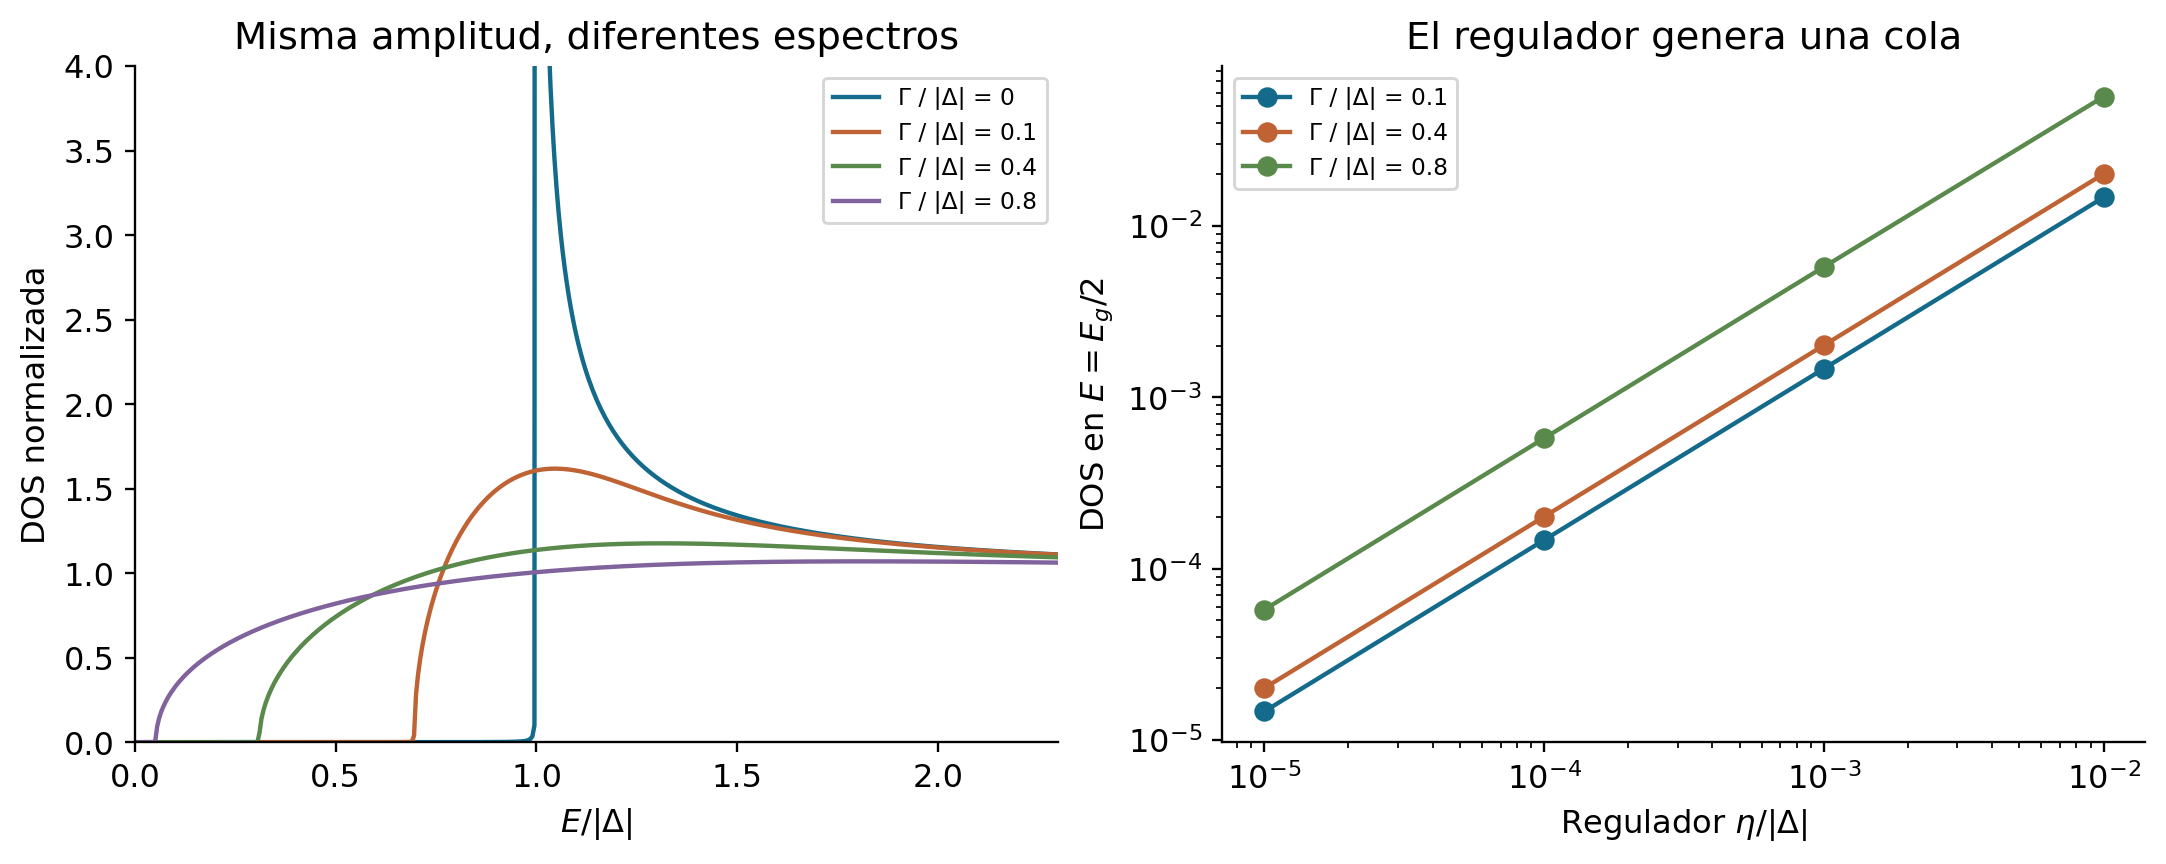
\includegraphics[width=0.96\linewidth,height=\textheight,keepaspectratio,alt={Resultado espectral de v0.4. Izquierda: DOS a amplitud fija y regulador \textbackslash eta/\textbar\textbackslash Delta\textbar=10\^{}\{-4\}. El máximo BCS supera el límite vertical elegido; se recorta su altura para mostrar los bordes y los otros espectros. Derecha: la DOS calculada por debajo del borde ideal disminuye al reducir el regulador.}]{../figuras/A_05_espectro_y_regulador.png}
\caption{Resultado espectral de v0.4. Izquierda: DOS a amplitud fija y
regulador \(\eta/|\Delta|=10^{-4}\). El máximo BCS supera el límite
vertical elegido; se recorta su altura para mostrar los bordes y los
otros espectros. Derecha: la DOS calculada por debajo del borde ideal
disminuye al reducir el regulador.}
\end{figure}

La lectura pedagógica es directa: \textbf{la amplitud puede mantenerse
igual y el acceso a estados cambiar mucho}. El panel derecho hace otra
distinción: una pequeña DOS bajo \(E_g\) puede ser efecto del regulador.
Al reducir \(\eta\) mil veces, esa contribución cae aproximadamente mil
veces en los tres casos mostrados; por tanto no se interpreta como una
población física nueva. Un ensanchamiento material medido exigiría otro
parámetro y otra justificación.

\section{A.4. Qué resultados se transfieren a cada
documento}\label{a.4.-quuxe9-resultados-se-transfieren-a-cada-documento}

La separación entre documentos también separa preguntas físicas: A
determina \textbf{el espectro y la energía estáticos}; B determina
\textbf{cómo se ocupan los estados y transportan energía}; C determina
\textbf{cómo evoluciona el condensado y se forma la señal}. El catálogo
de A se consulta a la amplitud y al superflujo presentes, sin imponer
(A.4) durante cada paso temporal.

{\def\LTcaptype{none} % do not increment counter
\begin{longtable}[]{@{}
  >{\raggedright\arraybackslash}p{(\linewidth - 2\tabcolsep) * \real{0.5000}}
  >{\raggedright\arraybackslash}p{(\linewidth - 2\tabcolsep) * \real{0.5000}}@{}}
\toprule\noalign{}
\begin{minipage}[b]{\linewidth}\raggedright
Resultado de A
\end{minipage} & \begin{minipage}[b]{\linewidth}\raggedright
Uso específico y destino
\end{minipage} \\
\midrule\noalign{}
\endhead
\bottomrule\noalign{}
\endlastfoot
(A.12), (A.16) y (A.19): energía libre y fuerza de amplitud & C.1--C.2:
extensión espacial experimental y ley del condensado. C.0 conecta esa
propuesta con la ecuación de la memoria. \\
(A.16): referencia normal y energía interna térmica & B.5.2: energía
térmica consistente. Sección C.4.2: energía de excitaciones y
temperatura equivalente. \\
(A.20)--(A.22): corriente como derivada e integrabilidad & C.12:
comparación de ramas y estabilidad uniforme. D: controles de derivadas y
convergencia. \\
(A.23)--(A.25): DOS, pesos anómalos y borde espectral & B.2--B.3:
soportes y coherencia de las colisiones; B.11: energía adiabática y
fuerzas de las ocupaciones. \\
(A.2) y (A.26)--(A.28): convenciones y restricciones materiales & B.6:
intercambio térmico con espectros materiales. D: trazabilidad y pruebas
antes de usar el catálogo. \\
\end{longtable}
}

La sección \textbf{B.11, «Energía adiabática y fuerzas de las
ocupaciones»}, distingue seguir estados de mantener una tabla fija en
energía. La sección \textbf{C.12} compara las ramas uniformes, conserva
la justificación de la corriente del cierre previo y evalúa las
modificaciones. Esos dos desarrollos permanecen en sus documentos
respectivos.

\textbf{La energía uniforme todavía no define una PDE válida en
cualquier punto.} Donde \(|\Delta|>0\), amplitud y fase permiten
consultar el catálogo local. En un cero del condensado,
\(\nabla\arg\Delta\) no está definido. Agregar solamente un costo
\(K_0|\nabla|\Delta||^2\) no garantiza una energía diferenciable en las
partes real e imaginaria de \(\Delta\), porque la rigidez de fase del
catálogo no coincide en general con ese \(K_0\). La regularización y la
energía espacial completa deben declararse juntas y derivarse antes de
discretizar. C.1--C.2 ensayan esa extensión; la comprobación uniforme de
A no certifica núcleos de vórtice, bordes ni recuperación de una región
normal.

\section{A.5. Material: por qué la corriente no fija toda la
energía}\label{a.5.-material-por-quuxe9-la-corriente-no-fija-toda-la-energuxeda}

\subsection{A.5.1. Qué significa el acoplamiento y qué significa el
límite
difusivo}\label{a.5.1.-quuxe9-significa-el-acoplamiento-y-quuxe9-significa-el-luxedmite-difusivo}

El \textbf{límite difusivo} describe el movimiento: las colisiones
elásticas cambian repetidamente la dirección electrónica antes de
recorrer las escalas superconductoras relevantes. Una condición usual es
\(\ell\ll\xi\), con camino libre medio \(\ell\) y longitud de coherencia
\(\xi\). La ecuación Usadel retiene la parte casi isotrópica del
propagador. El \textbf{acoplamiento débil} describe otra aproximación:
cómo se trata la interacción que empareja electrones y renormaliza su
espectro. En la referencia BCS isotrópica se obtiene
\(\Delta_0/(k_BT_c)=\pi e^{-\gamma_E}\simeq1.764\), donde \(\gamma_E\)
es la constante de Euler. Un material puede ser difusivo y necesitar
correcciones de acoplamiento fuerte.

En la convención energética de Eliashberg,

\[
\lambda=2\int_0^\infty\frac{\alpha^2F(\Omega)}{\Omega}\,d\Omega.
\tag{A.26}
\]

La memoria informa \(\lambda=1.216\) para el espectro NbN adoptado {[}M,
figura 4.6 y texto, p.~impresa 64{]}. Ese valor se cotejó en la fuente;
aquí no se recalcula la integral material. \(\lambda\) es un
\textbf{índice adimensional de intensidad del acoplamiento
electrón--fonón}, integrado sobre energías y estados electrónicos
relevantes. No es una probabilidad ni una fracción de pares: puede
superar uno. Un valor de orden unidad indica que la interacción no es un
parámetro pequeño que se pueda despreciar.

El factor \(1/\Omega\) permite leerlo: si dos bandas estrechas de
\(\alpha^2F\) tienen igual área y están centradas en \(\Omega_1\) y
\(2\Omega_1\), la primera aporta aproximadamente el doble a \(\lambda\).
Por eso conocer solo el área sin ponderar, o solo el número total de
modos de \(F\), no basta. A la inversa, dos espectros pueden tener el
mismo \(\lambda\) y distribuir el acoplamiento en energías diferentes.
Tampoco \(\lambda\) por sí solo fija \(T_c\) o la razón de gap:
intervienen la forma espectral y la repulsión electrónica efectiva. Las
clases de modos, DOS y DFPT del cuaderno E relacionan las vibraciones
con los pesos electrón--fonón.

Una interpretación adicional, en el caso isotrópico simple y de baja
energía, es la contribución electrón--fonón a la renormalización de
masa, \(m^*/m_{\rm banda}\simeq1+\lambda\). La excitación electrónica
arrastra una respuesta de la red y su dispersión cambia. Con
\(\lambda=1.216\) esa estimación sería \(2.216\), pero no constituye una
medida de la masa de la película ni una receta para multiplicar por ese
factor el \(N_0\) ya calibrado. La relación requiere su aproximación de
bandas y autoenergía {[}EPW{]}.

\subsection{A.5.2. Qué modifica Simon et al.~en el gap y por
qué}\label{a.5.2.-quuxe9-modifica-simon-et-al.-en-el-gap-y-por-quuxe9}

El apéndice \textbf{VII.3, «The Usadel equation», del preprint v3 de
{[}S{]}}, ecuaciones (11)--(14), usa Usadel con autoconsistencia BCS.
Después reescala resultados débiles por \(2.1/1.76\) para representar la
razón \(\Delta_0=2.1k_BT_c\) de NbN: la escala BCS sería demasiado
pequeña para esa elección material. Es una corrección práctica de escala
que conserva la forma espectral aproximada, no la solución completa de
Eliashberg. Los autores indican que esta última exigiría además una
ecuación para la renormalización y un gap dependiente de frecuencia.
\href{https://arxiv.org/html/2501.13791v3\#S7.SS3}{S, apéndice VII.3}

La consecuencia para este proyecto se ve directamente en (A.4). A
\(q=0\), su solución de acoplamiento débil fija la razón 1.764. Si se
reescala solamente el valor de salida \(|\Delta|\) manteniendo \(T_c\) y
la ecuación intactos, el valor reescalado ya no anula necesariamente
\(G\). Tampoco queda garantizado que la fuerza y la corriente
reescaladas sean derivadas de (A.12). Una aproximación empírica puede
ser útil, pero requiere declarar \textbf{qué magnitudes se reescalan} y
volver a comprobar (A.19)--(A.21).

Como sensibilidad algebraica, cambiar 1.764 por 2.1 aumenta el gap un
19.05\% y la escala \(N_0\Delta_0^2\) un 41.72\%, a \(N_0\) fijo. Son
consecuencias de multiplicar una escala y elevarla al cuadrado, no
predicciones nuevas para la película. Esa diferencia afecta justamente
la cantidad de energía necesaria para perturbar el condensado. Por eso
la razón 2.1 es una hipótesis material que se debe contrastar, mientras
(A.12) se mantiene como referencia débil verificable. Incorporar
\(\alpha^2F\) a las colisiones de B mejora esa parte microscópica; no
transforma automáticamente todo el catálogo estático en uno de
acoplamiento fuerte.

\subsection{A.5.3. Dos combinaciones distintas de
parámetros}\label{a.5.3.-dos-combinaciones-distintas-de-paruxe1metros}

Manteniendo \(T/T_c\) y la escala de gap fijos,

\[
j_{\rm dep}\propto\frac{\sigma_n}{\sqrt D},
\qquad C_{e,n}=\frac{2\pi^2}{3}N_0k_B^2T
\propto\frac{\sigma_n}{D}.
\tag{A.27}
\]

Calibrar \(D\) con una corriente restringe la primera combinación, pero
no constituye una medida independiente de la capacidad calorífica. Por
ejemplo, dos conjuntos que cumplan

\[
\frac{\sigma_{n,1}}{\sqrt{D_1}}
=\frac{\sigma_{n,2}}{\sqrt{D_2}}
\quad\Longrightarrow\quad
\frac{N_{0,1}}{N_{0,2}}=\sqrt{\frac{D_2}{D_1}}
\tag{A.28}
\]

pueden dar la misma escala de corriente y distinta energía electrónica.
Esta comparación algebraica reemplaza aquí una comparación entre
películas de procedencia no revalidada. La corriente de switching,
además, puede estar limitada por bordes o inhomogeneidades y no ser la
de depairing. La inductancia cinética dependiente de corriente aporta
una comprobación complementaria {[}Fr{]}.

\subsection{A.5.4. Entradas que necesitan restricciones
materiales}\label{a.5.4.-entradas-que-necesitan-restricciones-materiales}

{\def\LTcaptype{none} % do not increment counter
\begin{longtable}[]{@{}
  >{\raggedright\arraybackslash}p{(\linewidth - 4\tabcolsep) * \real{0.3333}}
  >{\raggedright\arraybackslash}p{(\linewidth - 4\tabcolsep) * \real{0.3333}}
  >{\raggedright\arraybackslash}p{(\linewidth - 4\tabcolsep) * \real{0.3333}}@{}}
\toprule\noalign{}
\begin{minipage}[b]{\linewidth}\raggedright
Entrada
\end{minipage} & \begin{minipage}[b]{\linewidth}\raggedright
Qué controla
\end{minipage} & \begin{minipage}[b]{\linewidth}\raggedright
Comprobación propuesta
\end{minipage} \\
\midrule\noalign{}
\endhead
\bottomrule\noalign{}
\endlastfoot
\(D\) & Difusión, ruptura de pares y \(N_0\) inferido & Transporte y,
cuando corresponda, pendiente de \(H_{c2}\) \\
\(\sigma_n\), \(d\) & Escala de corriente y conversión de resistencia de
hoja & Resistencia y espesor de la misma película \\
\(\Delta(T)\) & Espectro y energía de emparejamiento & Espectroscopia o
catálogo material consistente \\
\(N_0\) & Energía y capacidad electrónicas & Capacidad normal o
información electrónica independiente \\
\(F\), \(\alpha^2F\), \(N_i\) & Colisiones y energía fonónica & Fase,
estequiometría y normalización por átomo, fórmula o celda \\
Tiempos efectivos & Relajación, cascada y escape & Precisar el proceso
que representa cada tiempo \\
\end{longtable}
}

\section{A.6. Decisión de modelamiento para esta
iteración}\label{a.6.-decisiuxf3n-de-modelamiento-para-esta-iteraciuxf3n}

Se adopta como \textbf{referencia uniforme verificable} el funcional
Usadel de acoplamiento débil (A.12) y sus fuerzas conjugadas. Sus
salidas alimentan la extensión no térmica adiabática de B.11 y la
dinámica de C. Esta organización permite comprobar cada aproximación
donde se introduce.

La prioridad es comprobar las identidades, los límites BCS/GL y las
curvas uniformes antes de conectar el catálogo con una dinámica
espacial. La ley de relajación del condensado y la transición desde la
cinética no térmica al cierre reducido requieren sus propias pruebas,
descritas en B--D. No se cambia aquí el solver de producción ni se
atribuyen nuevas latencias al detector.

Si los datos de la película requieren acoplamiento fuerte, el catálogo
puede ampliarse con autoenergías dependientes de energía. Proyectar ese
campo de emparejamiento espectral sobre una sola amplitud necesita una
definición adicional; esa ampliación no se declara deducida ni
implementada en v0.4. Su necesidad se decidirá por la precisión
requerida y las restricciones materiales disponibles. El ajuste de Simon
es un antecedente concreto para estudiar esa aproximación, no una
identidad adicional del funcional actual.

\subsection{A.6.1. Verificación independiente de esta
revisión}\label{a.6.1.-verificaciuxf3n-independiente-de-esta-revisiuxf3n}

Se resolvieron \textbf{80 estados}:
\(T/T_c\in\{0.05,0.15,0.4,0.8,0.98\}\),
\(|\Delta|/(k_BT_c)\in\{0.25,0.8,1.5,2\}\) y
\(Q\in\{0,0.15,0.45,0.75\}\). El script nuevo resuelve la energía de
Matsubara renormalizada por Newton acotado; no importa el solver de
producción ni el cálculo anterior. Se usan sumas crudas con 128 a 8192
frecuencias y extrapolación al retirar el corte, en lugar de reutilizar
la corrección analítica de cola de v0.3.

Las pendientes se contrastan por diferencias finitas de cuarto orden con
cinco pasos, de \(10^{-2}\) a \(10^{-4}\). Las variables y la energía se
adimensionalizan con \(k_BT_c\) y \(N_0(k_BT_c)^2\). Para una cantidad
de referencia \(r\), el error mostrado es
\(|r_{\rm num}-r|/\max(1,|r|)\); en la identidad de derivadas mixtas se
usa el mayor módulo de ambas. Esta escala sigue siendo interpretable
cuando la corriente o una fuerza es cero.

\begin{figure}
\centering
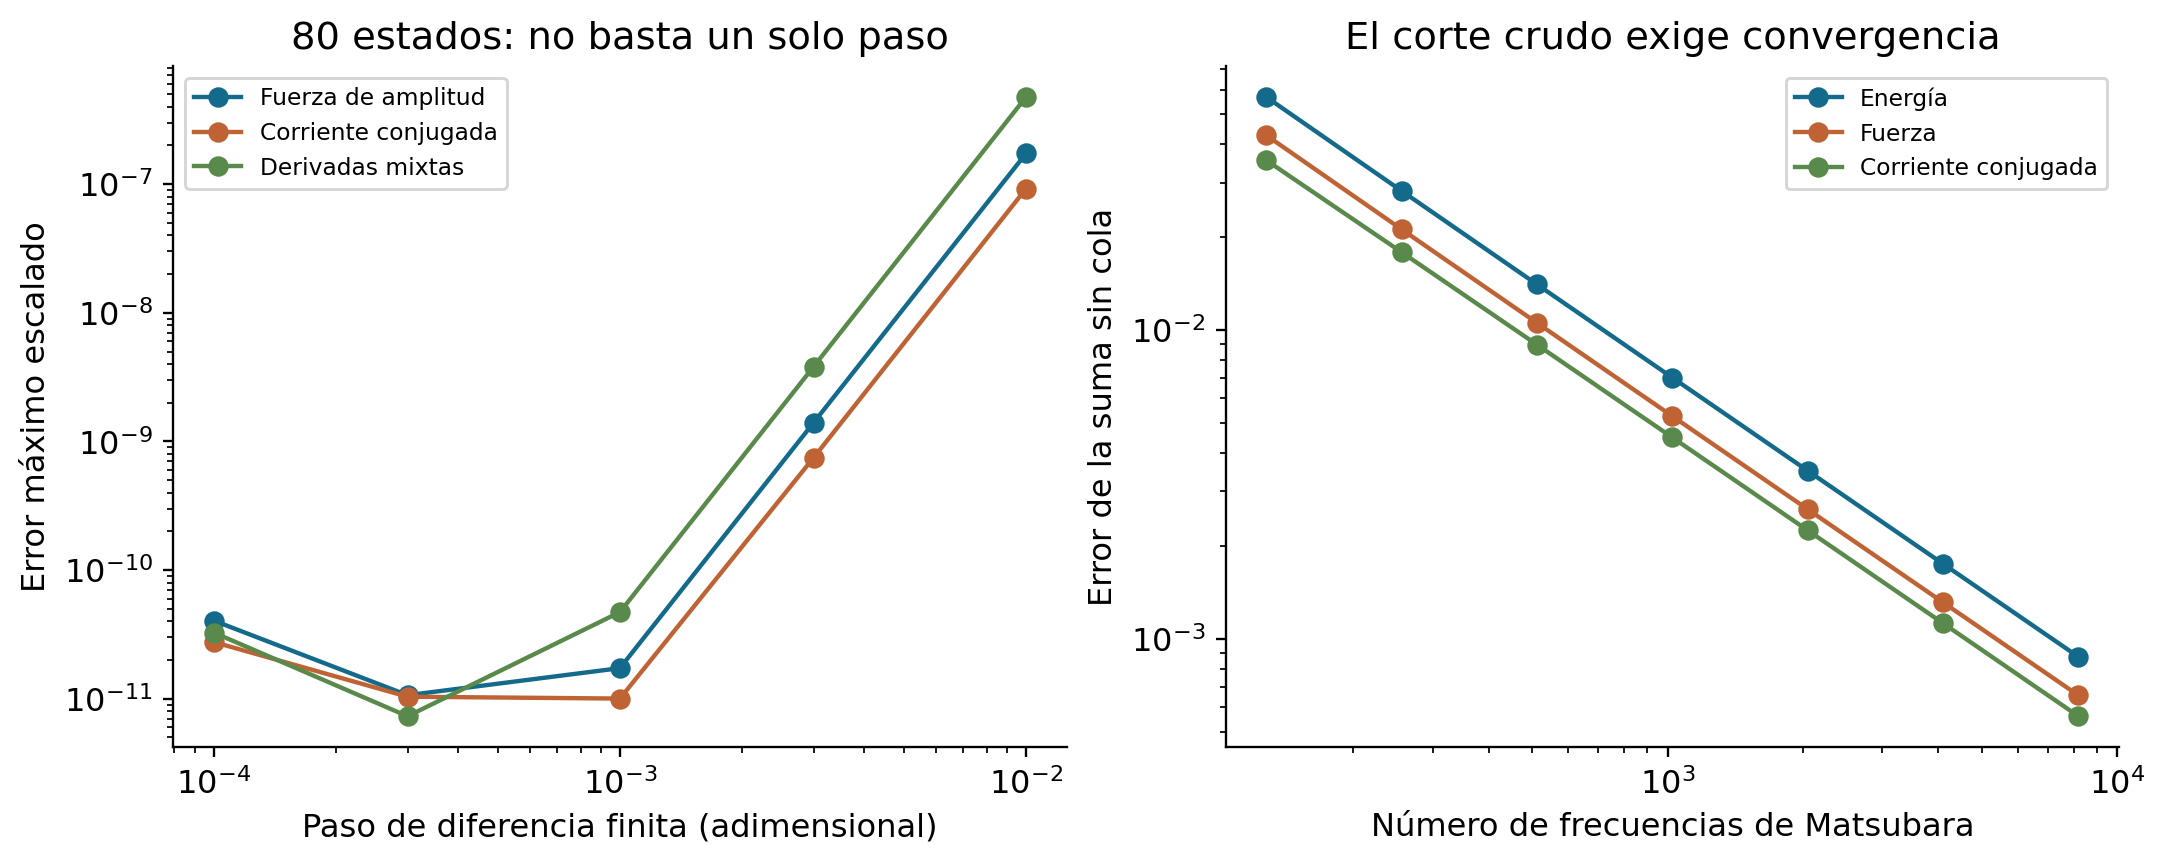
\includegraphics[width=0.96\linewidth,height=\textheight,keepaspectratio,alt={Auditoría calculada en Geminga. Izquierda: máximo error de derivación sobre los 80 estados al cambiar el paso. Derecha: error máximo de las sumas crudas frente a la extrapolación. Derivar con precisión una suma truncada no elimina su error de corte.}]{../figuras/A_04_auditoria_independiente.png}
\caption{Auditoría calculada en Geminga. Izquierda: máximo error de
derivación sobre los 80 estados al cambiar el paso. Derecha: error
máximo de las sumas crudas frente a la extrapolación. Derivar con
precisión una suma truncada no elimina su error de corte.}
\end{figure}

{\def\LTcaptype{none} % do not increment counter
\begin{longtable}[]{@{}
  >{\raggedright\arraybackslash}p{(\linewidth - 2\tabcolsep) * \real{0.5000}}
  >{\raggedright\arraybackslash}p{(\linewidth - 2\tabcolsep) * \real{0.5000}}@{}}
\toprule\noalign{}
\begin{minipage}[b]{\linewidth}\raggedright
Comprobación
\end{minipage} & \begin{minipage}[b]{\linewidth}\raggedright
Resultado máximo en la malla
\end{minipage} \\
\midrule\noalign{}
\endhead
\bottomrule\noalign{}
\endlastfoot
Fuerza de amplitud frente a derivada de energía, paso \(10^{-3}\) &
\(1.73\times10^{-11}\), error escalado \\
Corriente conjugada frente a derivada de energía, mismo paso &
\(1.00\times10^{-11}\), error escalado \\
Identidad de derivadas mixtas, mismo paso & \(4.71\times10^{-11}\),
error escalado \\
Cambio al desplazar la ventana de extrapolación de cortes &
\(3.16\times10^{-12}\), error escalado de energía o derivadas \\
Residuo retardado, 12020 combinaciones de energía, ruptura de pares y
regulador & \(2.34\times10^{-14}\), escalado por energía \\
Normalización \(|(c^R)^2+(s^R)^2-1|\) & \(7.28\times10^{-12}\) \\
\end{longtable}
}

La extrapolación ajusta un polinomio de cuarto grado en el inverso del
número de frecuencias; se comparan las ventanas
\(\{256,512,1024,2048,4096\}\) y \(\{512,1024,2048,4096,8192\}\). El
cambio entre ventanas mide estabilidad numérica, no una cota matemática
del error total. En el espectro se ensayaron \(E/|\Delta|\) entre 0 y 3,
\(\Gamma/|\Delta|\in\{0,0.1,0.4,0.8,1.1\}\) y los cuatro reguladores de
la sección A.3.2; la DOS fue no negativa. Maximizar numéricamente la
rama subgap reprodujo el borde (A.25) con error menor que
\(10^{-10}|\Delta|\) en los tres casos intermedios.

\textbf{Conclusión de la prueba.} Las identidades estáticas sobreviven a
un método espectral y una retirada del corte diferentes de los usados
antes. El mínimo del error al variar el paso muestra también dónde
empieza a dominar el redondeo. Estas pruebas detectan errores de
normalización, derivación, rama causal o truncación antes de un
transitorio; no anticipan por sí solas su latencia, estabilidad espacial
o balance de energía completo. La regularidad de la energía espacial y
las colisiones requieren los ensayos de B--D.

\section{Referencias y procedencia}\label{referencias-y-procedencia}

{[}M{]} J. A. Díaz Monge, \emph{Multiscale Modeling of the Transient
Response of Superconducting Nanowire Single-Photon Detectors},
Universidad de Chile, 2026. Copia cotejada: \nolinkurl{memoria_02.pdf},
173 páginas, obtenida de
\nolinkurl{/home/jdiaz/memoria/main/memoria_02.pdf} en Geminga. Ver A.5,
p.~impresa 112 (página 143 del PDF), para el cierre de corriente; C.2,
pp.~impresas 121--123 (páginas 152--154 del PDF), ecuaciones
(C.4)--(C.10), para la cancelación de divergencias. El archivo local de
nombre \nolinkurl{Memoria_JDiaz_JF_v0.pdf} corresponde a otra copia y no
se usa para atribuir esta paginación.

{[}V{]} D. Y. Vodolazov, \emph{Single-Photon Detection by a Dirty
Current-Carrying Superconducting Strip Based on the Kinetic-Equation
Approach}, Physical Review Applied \textbf{7}, 034014 (2017).
\href{https://doi.org/10.1103/PhysRevApplied.7.034014}{Artículo, DOI};
\href{https://arxiv.org/pdf/1611.06060}{preprint completo}. Ver
ecuaciones (33)--(37), pp.~10--11 del PDF: corriente, corrección del RHS
y continuidad. Se ha cotejado específicamente p.~11, ecuación (36).

{[}F{]} P. Virtanen, A. Vargunin y M. Silaev, \emph{Quasiclassical free
energy of superconductors: Disorder-driven first-order phase transition
in superconductor/ferromagnetic-insulator bilayers}, Physical Review B
\textbf{101}, 094507 (2020).
\href{https://doi.org/10.1103/PhysRevB.101.094507}{DOI};
\href{https://jyx.jyu.fi/bitstreams/f577693c-c6d1-4923-866c-353ec3ac8dd5/download}{copia
institucional};
\href{https://arxiv.org/pdf/1909.00992}{arXiv:1909.00992}. La derivación
parte de la ecuación (20), p.~094507-3; el preprint v1 conserva esa
numeración, p.~3, bajo el título \emph{Quasiclassical expressions for
the free energy of superconducting systems}. Se corrige el título
bibliográfico de la revisión 0.1.

{[}S{]} A. Simon et al., \emph{Ab initio modeling of nonequilibrium
dynamics in superconducting detectors and qubits}, Physical Review B
\textbf{112}, 174512 (2025).
\href{https://journals.aps.org/prb/abstract/10.1103/3m2k-mzr6}{Ficha
editorial y DOI};
\href{https://arxiv.org/html/2501.13791v3\#S7.SS3}{preprint v3, apéndice
VII.3}. La identidad bibliográfica se cotejó en APS; la numeración del
apéndice y la explicación del reescalamiento se cotejaron en el
preprint. No se atribuye esa paginación al PDF publicado.

{[}EPW{]} F. Giustino, material docente de la \emph{Summer School on
Electron--Phonon Physics}, 2022, diapositiva 24: relación entre
pendiente de la autoenergía y renormalización de masa, con el alcance
del caso simple indicado en la fuente.
\href{https://docs.epw-code.org/_downloads/720916b4aba43b13d75d323126c36a0c/Tue.2.Giustino.pdf}{Apuntes
oficiales EPW}.

{[}Fr{]} S. Frasca et al., \emph{Determining the depairing current in
superconducting nanowire single-photon detectors}, Physical Review B
\textbf{100}, 054520 (2019).
\href{https://doi.org/10.1103/PhysRevB.100.054520}{DOI}.

{[}R{]} Repositorio \nolinkurl{pysnspd}, rama \nolinkurl{main}; cálculo
uniforme independiente de esta revisión:
\nolinkurl{sandbox/model_v0_4/checks_a_v04.py}. D registra la base de
código, la ejecución en Geminga, los resultados y la procedencia
completa. Las cuatro figuras se generaron de nuevo con ese cálculo. Los
CSV y el informe \nolinkurl{A_auditoria_independiente_v04.json}, en
\nolinkurl{verificaciones/}, conservan las mallas y resultados;
\nolinkurl{A_mapa_ecuaciones.json} registra la auditoría de numeración.

\end{document}
